\section{实验设计}
\subsection{ALU}\label{sub:alu}
\subsubsection{功能描述}
该 ALU 实现加法、减法、按位与、按位或、取反及无符号小于判断等基础运算功能,支持 8 位
与 32 位输入,输出 32 位结果,并在数码管上进行显示。
\subsubsection{接口定义}
\begin{table}[htp]
\caption{接口定义}\label{tab:signaldef}
\begin{center}
	\begin{tabular}{|l|l|l|p{6cm}|}
	\hline
	\textbf{信号名} & \textbf{方向} & \textbf{位宽} & \textbf{功能描述}\\ \hline \hline
	num1	&Input	&8-bit	&操作数1\\
	num2	&Input	&32-bits	& 操作数2\\
	op	&Output	&3-bits	& 操作码\\
	result	&Output	&32-bits & 计算结果\\
	seg &Output &7-bits & 七段数码管\\
	clk &Input &1-bit & 时钟信号\\
	reset &Input &1-bit & 复位信号\\
	\hline
	\end{tabular}
\end{center}
\end{table}

\subsubsection{逻辑控制}
本 ALU 模块采用组合逻辑控制方式,不使用时序触发的有限状态机(FSM)。由于 ALU 
运算为即时反应型逻辑(无时序依赖),其控制流程可简化为单周期组合逻辑响应,无需状态跳转。
模块通过将 8 位输入零扩展为 32 位,并根据 3 位操作码执行加、减、与、或、取反和小于判断等运算,非法操作码输出全 x。
ALU的控制逻辑使用组合逻辑电路实现,具体如下:
\begin{figure}[htbp]
    \centering
    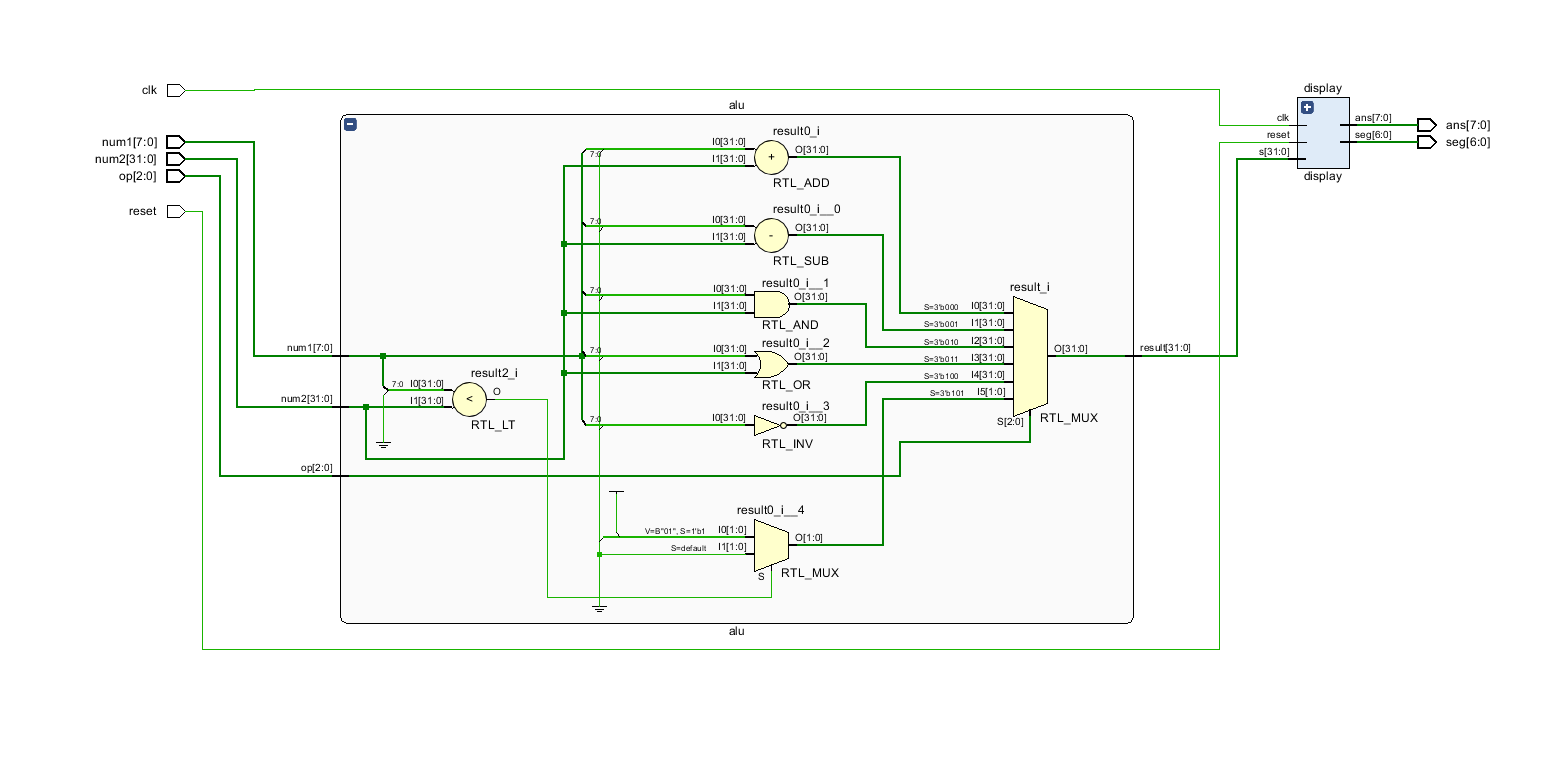
\includegraphics[width=0.7\textwidth]{image/yingjian.png}
    \caption{ALU控制逻辑电路}
	\label{fig:alu_control}
\end{figure}
\subsection{有阻塞4级8bit全加器}\label{sub:ctl}
\subsubsection{功能描述}
本模块 \texttt{adder} 是一个采用四级流水线结构实现的 32 位加法器。模块接收两个 32 位输入操作数 \texttt{num1} 和 \texttt{num2},通过每阶段处理 8 位数据逐步完成加法,并支持输入初始进位 \texttt{cin}。模块支持异步复位 \texttt{reset},每级流水线的刷新控制 \texttt{refresh} 以及暂停控制 \texttt{stop},并提供各阶段调试输出与流水线状态指示。最终输出结果为 32 位加法结果 \texttt{ans} 和最终进位 \texttt{cout}。

\subsubsection{接口定义}
\text{}见下表
\begin{table}[htp]
	\caption{adder 模块接口定义}\label{tab:adder_interface}
	\begin{center}
		\begin{tabular}{|l|l|l|p{6cm}|}
		\hline
		\textbf{信号名} & \textbf{方向} & \textbf{位宽} & \textbf{功能描述} \\ \hline \hline
		clk             & Input  & 1     & 时钟信号,驱动流水线各阶段时序逻辑 \\
		reset           & Input  & 1     & 异步复位信号,高电平有效,清除所有状态 \\
	refresh         & Input  & 4     & 各流水线级刷新信号,高电平有效清除对应阶段状态 \\
	stop            & Input  & 4     & 各流水线级暂停信号,高电平阻止流水前传 \\
	cin             & Input  & 1     & 初始加法进位 \\
	validin         & Input  & 1     & 输入数据有效标志 \\
	out\_allow      & Input  & 1     & 输出允许信号,决定是否将结果输出 \\
	num1            & Input  & 32    & 加法器第一个操作数 \\
	num2            & Input  & 32    & 加法器第二个操作数 \\
	validout        & Output & 1     & 输出数据有效标志,表示结果已准备好 \\
	ans             & Output & 32    & 最终加法结果 \\
	cout            & Output & 1     & 最终进位输出 \\
	debug\_sum1     & Output & 8     & 第一阶段的部分加法结果(用于Debug) \\
	debug\_sum2     & Output & 16    & 第二阶段的部分加法结果(用于Debug) \\
	debug\_sum3     & Output & 24    & 第三阶段的部分加法结果(用于Debug) \\
	debug\_sum4     & Output & 32    & 第四阶段(最终)的加法结果(用于Debug) \\
	pipe1\_valid\_out & Output & 1    & 第一阶段有效状态指示 \\
	pipe2\_valid\_out & Output & 1    & 第二阶段有效状态指示 \\
	pipe3\_valid\_out & Output & 1    & 第三阶段有效状态指示 \\
	pipe4\_valid\_out & Output & 1    & 第四阶段有效状态指示 \\
		\hline
		\end{tabular}
	\end{center}
	\end{table}
\subsubsection{逻辑控制}

本模块采用四级流水线结构,逐步完成 32 位加法操作,每级处理 8 位数据,并传递进位信息,详细逻辑如下:

\begin{itemize}
    \item \textbf{流水线允许控制}:每一级通过 \texttt{allowin} 信号判断是否能接收数据,条件为本级未被 \texttt{stop[i]} 阻塞,且下一级允许传输数据,或本级当前无效。
    
    \item \textbf{数据传递与寄存}:每一阶段使用寄存器保存当前级别的部分和与操作数剩余高位,下一阶段继续处理更高位加法并拼接形成完整结果。
    
    \item \textbf{进位传递逻辑}:初始进位 \texttt{cin} 输入到第一阶段,后续每级进位通过前一级的进位累加传递。
    
    \item \textbf{复位与刷新机制}:模块支持复位信号 \texttt{reset},用于清除所有阶段的 \texttt{valid} 状态。单独阶段可通过对应的 \texttt{refresh[i]} 控制信号进行刷新清除。
    
    \item \textbf{输出控制}:最终输出由第四级流水线完成,其输出受 \texttt{out\_allow} 控制。若该阶段有效且输出允许,则输出 \texttt{ans} 和 \texttt{cout},同时置 \texttt{validout} 为高。
    
    \item \textbf{调试输出}:模块提供每一级流水的调试输出 \texttt{debug\_sum*},用于观察中间和的变化情况,辅助调试与验证。
\end{itemize}
